\documentclass{scrartcl}
\documentclass[tikz]{standalone}

\usepackage{tkz-euclide}
\usepackage{graphicx} % Required for inserting images
\usepackage{amsmath}
\usepackage{listings}
\usepackage{evan}
\usepackage{changepage}
\usepackage{asymptote}
\usepackage{setspace}

\setstretch{1.25}
\title{2025 AIME I Solutions}
\author{Raine Ma}

\begin{document}
\maketitle

These solutions are just how I solved the problem in-contest, and are not necessarily the best or most efficient way to approach them. 

\section*{Problem 1}

\textbf{Find the sum of all integer bases $b>9$ for which $17_b$ is a divisor of $97_b.$}\\

We are given that
$$9b+7 \equiv 0~(\text{mod }b+7)$$
We can easily eliminate the $b$ by subtracting $9(b+7)$.

$$9b+7 - 9b - 63 \equiv 0~(\text{mod } b+7)$$

$$-56 \equiv 0~(\text{mod } b+7)$$

The divisors of 56 are $\{1, 2, 4, 7, 8, 14, 28, 56\}$. Trying from these values, we find that only $b=21,49$ works. Therefore, the desired sum is $21+49 = $ $$\boxed{070}$$

\newpage

\section*{Problem 2}

\textbf{$\triangle ABC$ points $D$ and $E$ lie on $\overline{AB}$ so that $AD < AE < AB$, while points $F$ and $G$ lie on $\overline{AC}$ so that $AF < AG < AC$. Suppose $AD = 4$, $DE = 16$, $EB = 8$, $AF = 13$, $FG = 52$, and $GC = 26$. Let $M$ be the reflection of $D$ through $F$, and let $N$ be the reflection of $G$ through $E$. The area of quadrilateral $DEGF$ is $288$. Find the area of heptagon $AFNBCEM$, as shown in the figure below.}\\

\begin{asy}
unitsize(14);
pair A = (0, 9), B = (-6, 0), C = (12, 0), D = (5A + 2B)/7, E = (2A + 5B)/7, F = (5A + 2C)/7, G = (2A + 5C)/7, M = 2F - D, N = 2E - G;
filldraw(A--F--N--B--C--E--M--cycle, lightgray);
draw(A--B--C--cycle);
draw(D--M);
draw(N--G);
dot(A);
dot(B);
dot(C);
dot(D);
dot(E);
dot(F);
dot(G);
dot(M);
dot(N);
label("$A$", A, dir(90));
label("$B$", B, dir(225));
label("$C$", C, dir(315));
label("$D$", D, dir(135));
label("$E$", E, dir(135));
label("$F$", F, dir(45));
label("$G$", G, dir(45));
label("$M$", M, dir(45));
label("$N$", N, dir(135));
\end{asy}\\

Through the area of a trapezoid, and by inspection, we have $$[ADF]=[AFM], [DEGF]=[FNEM], \& [EBCG]=[NBCE]$$. Then, it follows that $$[AFNBCEM]=[ABC]$$ Given $AD:DE:EB=1:4:2$, we have $$\frac{[DEGF]}{[ABC]}=\frac{5^2-1^2}{7^2}=\frac{24}{49}$$Then $$[AFNBCEM]=[ABC]=\frac{49}{24}\cdot[DEGF]=\frac{49}{24}\cdot 288=\boxed{588}$$

\newpage

\section*{Problem 3}

\textbf{The 9 members of a baseball team went to an ice-cream parlor after their game. Each player had a singlescoop cone of chocolate, vanilla, or strawberry ice cream. At least one player chose each flavor, and the number of players who chose chocolate was greater than the number of players who chose vanilla, which was greater than the number of players who chose strawberry. Let $N$ be the number of different assignments of flavors to players that meet these conditions. Find the remainder when $N$ is divided by $1000.$}\\

Denote $C,V,S$ as chocolate, vanilla, and strawberry respectively. We wish to find $(C,V,S)$ such that $C>V>S>0$. \\

Let $C=s+v+c$, $V=s+v$, $S=s$, and $c,v,s\geq1$. Observe that this satisfies the problem constraints. Then we have $c+2v+3s=9$. We wish to find the ordered triples $(c,v,s)$ that satisfy this equation, and then substitute this back in. \\

\subsubsection*{Case 1: $s=1$}
\begin{adjustwidth}{2.5em}{0pt}
$c+2v = 6$\\
The solutions are $(4,1,1)$ and $(2,2,1)$\\
\end{adjustwidth}

\subsubsection*{Case 2: $s=2$}
\begin{adjustwidth}{2.5em}{0pt}
$c+2v = 3$\\
$(1,1,2)$ is the only solution. The case $s=3$ is impossible based on our constraints.\\
\end{adjustwidth}


Substituting back in, we find the possible ordered triples $(C,V,S)$ are $(6,2,1),(5,3,1),(4,3,2)$. Then, we count the combinations:

$$\binom{9}{6,2,1} + \binom{9}{5,3,1} + \binom{9}{4,3,2}$$

$$= 252 + 504 + 1260 = 2016$$

Since the problem asks us to find $(\text{mod } 1000)$, the answer is $$\boxed{016}$$



\newpage

\section*{Problem 4}

\textbf{Find the number of ordered pairs $(x,y)$, where both $x$ and $y$ are integers between $-100$ and $100$ inclusive, such that $12x^2-xy-6y^2=0$.}\\

We factor the expression:
$$12x^2 + 8xy - 9xy - 6y^2 = 0$$

$$(4x-3y)(3x+2y) = 0$$

Therefore, there are 2 cases. 

\subsubsection*{Case 1: $4x-3y=0$}

\begin{adjustwidth}{2.5em}{0pt}
We have $y=\frac{4}{3}x$.
Therefore, $y$ can be any value divisible by 4 in the range $[-100,100]$. There are $51$ such values, and each value of $y$ gives a unique value for $x$, ensuring uniqueness. 
\end{adjustwidth}
\subsubsection*{Case 2: $s=2$}
\begin{adjustwidth}{2.5em}{0pt}
We have $y=-\frac{3}{2}x$.
Therefore, $y$ can be any value divisible by 3 in the range $[-100,100]$. There are $67$ such values.\\

\end{adjustwidth}

However, we have overcounted the case $(0,0)$. This can be seen by noting the lines intersect here, or intuition. Therefore, the answer is $$51+67-1 = \boxed{117}$$ 

\newpage

\section*{Problem 5}

\textbf{There are $8!= 40320$ eight-digit positive integers that use each of the digits 1, 2, 3, 4, 5, 6, 7, 8 exactly once. Let N be the number of these integers that are divisible by $22$. Find the difference between $N$ and 2025.}\\

For a number to be divisible by 11, the difference between the sum of digits at even and odd positions must be 0 or a multiple of 11. It is easy to see that the difference here must be 0. \\

The sum of the digits is $\frac{8\cdot 9}{2} = 36$. Therefore, we wish to find all $(A,B,C,D)$ such that $1\leq A<B<C<D\leq8$ and $A+B+C+D=18$.\\

Let $A=x_1$, $B=x_1+x_2$, $C=x_1+x_2+x_3$, and $D=x_1+x_2+x_3+x_4$. \\

Then $4x_1+3x_2+2x_3+x_4 = 18$. \\

Substitute $y_i = x_i - 1$ to eliminate the $\geq1$ condition:\\

$4y_1+3y_2+2y_3+y_4 = 8$\\

Casework reveals 8 solutions, namely: $$(0,0,4,0),(0,1,2,1),(0,2,0,2),(0,2,1,0),(1,0,1,2),(1,0,2,0),(1,1,0,1),(2,0,0,0)$$. 

Now, once we choose which set we want to use, the other 4 numbers are fixed. There are $4!$ ways to permute each set. However, we have overcounted, as the last digit must be even. By symmetry, this eliminates exactly half of the solutions.\\ Therefore, the answer is $$\frac{8\cdot(4!)^2}{2} = 2304 - 2025 = \boxed{279}$$
\newpage

\section*{Problem 6}

\textbf{An isosceles trapezoid has an inscribed circle tangent to each of its four sides. The radius of the circle is $3$, and the area of the trapezoid is $72$. Let the parallel sides of the trapezoid have lengths $r$ and $s$, with $r \neq s$. Find $r^2+s^2$.}\\

\textbf{Diagram}

\begin{asy}
unitsize(0.5 cm);

real r_base = 12 + 6*sqrt(3); 
real s_base = 12 - 6*sqrt(3); 
real h = 6;  

pair A = (-r_base/2, 0);
pair B = ( r_base/2, 0);
pair C = ( s_base/2, h);
pair D = (-s_base/2, h);

draw(A--B--C--D--cycle);

pair O = (0, h/2);
draw(circle(O, 3));

dot(A); label("$A$", A, SW);
dot(B); label("$B$", B, SE);
dot(C); label("$C$", C, NE);
dot(D); label("$D$", D, NW);

dot(O);

draw((0,0)--(0,h), dashed+linewidth(1));
label("$O$", (0,h/2), E);

label("$r$", midpoint(A--B), S);
label("$s$", midpoint(C--D), N);
\end{asy}

First, we use the area of a trapezoid formula:\\

$\frac{1}{2}\cdot(r+s)\cdot6 = 72 \implies r+s = 24$\\

A nice property of tangential quadrilaterals are that the sums of opposite sides are equal. Therefore, the two legs each have length 12, since tangents from a point have equal length. \\

Then, by the Pythagorean Theorem, 

$$\frac{r-s}{2} = \sqrt{12^2 - 6^2} = 6\sqrt{3} \implies r-s = 12\sqrt{3}$$

$$2(r^2 + s^2) = (r+s)^2 + (r-s)^2 = 576 + 432 = 1008$$
Therefore,
$$r^2+s^2 = \boxed{504}$$

\newpage

\section*{Problem 7}

\textbf{The twelve letters $A$,$B$,$C$,$D$,$E$,$F$,$G$,$H$,$I$,$J$,$K$, and $L$ are randomly grouped into six pairs of letters. The two letters in each pair are placed next to each other in alphabetical order to form six two-letter words, and then those six words are listed alphabetically. For example, a possible result is $AB$, $CJ$, $DG$, $EK$, $FL$, $HI$. The probability that the last word listed contains $G$ is $\frac mn$, where $m$ and $n$ are relatively prime positive integers. Find $m+n$.}\\

Observe that there are two cases, either $G$ is the first letter in the last pair, or that $G$ is the second letter in the last pair.


\subsubsection*{Case 1: G is the first letter}
\begin{adjustwidth}{2.5em}{0pt}

There are $5$ choices for the letter immediately following $G$, namely $HIJKL$.\\

Assume, WLOG, that we pick $H$. Then we have $ABCDEF IJKL$ left. \\

There are $\binom{6}{4} = 15$ ways to pair up $IJKL$ with letters from $ABCDEF$. The remaining $2$ letters are forced to pair up. Then, there are also $4!$ ways to permute $IJKL$. \\

Using construction, there are $5\cdot\binom{6}{4}\cdot5!$ solutions in this case. 

\end{adjustwidth}

\subsubsection*{Case 2: G is the second letter}
\begin{adjustwidth}{2.5em}{0pt}

The first letters must be $A,B,C,D,E,F$. The last pair must be $FG$, however, the second letter may be any letter from $HIJKL$ the first $5$. Therefore, there are $5!$ solutions in the case. \\
\end{adjustwidth}
There are $$\binom{12}{2}\cdot\binom{10}{2}\cdot\binom{8}{2}\cdot\binom{6}{2}\cdot\binom{4}{2}$$ ways to choose the groups, however we must divide by $6!$ since the order does not matter. Therefore, the denominator is $$\frac{\binom{12}{2}\cdot\binom{10}{2}\cdot\binom{8}{2}\cdot\binom{6}{2}\cdot\binom{4}{2}}{6!} = \frac{66\cdot45\cdot28\cdot15\cdot6}{720} = 33\cdot45\cdot7$$

Therefore, the answer is $$\frac{1920}{10895} = \frac{128}{693} = \boxed{821}$$

I sillied this one (failed arithmetic) :(

\newpage

\section*{Problem 8}

\textbf{Let $k$ be a real number such that the system \begin{align*} |25+20i-z|&=5\\ |z-4-k|&=|z-3i-k| \end{align*} has exactly one complex solution $z.$ The sum of all possible values of $k$ can be written as $\dfrac{m}{n},$ where $m$ and $n$ are relatively prime positive integers. Find $m+n.$ Here $i=\sqrt{-1}.$}\\
\begin{center}
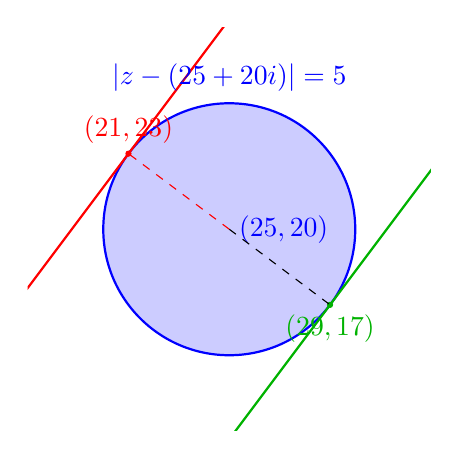
\begin{tikzpicture}[scale=0.32]
  % Draw coordinate axes

  \clip (17,12) rectangle (33,28);

  
  \draw[->] (0,0) -- (40,0) node[right] {$x$};
  \draw[->] (0,0) -- (0,35) node[above] {$y$};

  %-----------------------------
  % Draw the circle |25+20i-z|=5
  % (Note: The circle’s center is (25,20) because |25+20i-z| = |z-(25+20i)|.)
  \filldraw[fill=blue!20, draw=blue, thick] (25,20) circle (5);
  \node[blue, right] at (25,20) {$(25,20)$};

  %-----------------------------
  % For k = 23/8:
  % Compute the endpoints of the segment (which determine the bisector).
  % The two fixed points are: A = (4+k,0) and B = (k,3).
  \def\kone{23/8}
  \coordinate (A1) at ({4+\kone},0);  % (4 + 23/8, 0)
  \coordinate (B1) at ({\kone},3);     % (23/8, 3)
  % Draw the points and label them.
  \filldraw[red] (A1) circle (0.5) node[below] {$\left(4+\frac{23}{8},0\right)$};
  \filldraw[red] (B1) circle (0.5) node[above left] {$\left(\frac{23}{8},3\right)$};
  % Connect them by a dotted segment.
  \draw[red,dotted,thick] (A1) -- (B1);
  
  % The perpendicular bisector of the segment joining A1 and B1 is
  % given by 8x - 6y - 8k - 7 = 0. For k = 23/8, this becomes:
  %   8x - 6y - 8*(23/8) - 7 = 8x - 6y -23 -7 = 8x - 6y -30 = 0,
  % which can be rewritten as y = (4/3)x - 5.
  \draw[red, thick, domain=0:40] 
       plot (\x, { (4/3)*\x - 5}) 
       node[right] {$8x-6y-30=0,\quad k=\frac{23}{8}$};
       
  % The tangency point is the projection of the circle’s center (25,20)
  % onto this line. (A short computation shows it is (21,23).)
  \filldraw[red] (21,23) circle (0.1) node[above] {$(21,23)$};
  \draw[dashed, red] (25,20) -- (21,23);
  
  %-----------------------------
  % For k = 123/8:
  \def\ktwo{123/8}
  \coordinate (A2) at ({4+\ktwo},0);  % (4 + 123/8, 0)
  \coordinate (B2) at ({\ktwo},3);     % (123/8, 3)
  \filldraw[green!70!black] (A2) circle (0.5) 
       node[below] {$\left(4+\frac{123}{8},0\right)$};
  \filldraw[green!70!black] (B2) circle (0.5) 
       node[above left] {$\left(\frac{123}{8},3\right)$};
  \draw[green!70!black,dotted,thick] (A2) -- (B2);
  
  % Now the perpendicular bisector for these points:
  % For k = 123/8 the equation becomes:
  %   8x - 6y - 8*(123/8) - 7 = 8x - 6y -123 -7 = 8x -6y -130 = 0,
  % i.e. y = (4/3)x - (130/6) = (4/3)x - 65/3.
  \draw[green!70!black, thick, domain=0:40] 
       plot (\x, { (4/3)*\x - 65/3}) 
       node[right] {$8x-6y-130=0,\quad k=\frac{123}{8}$};
  
  % Its tangency point with the circle (projection of (25,20) onto the line)
  % works out to be (29,17).
  \filldraw[green!70!black] (29,17) circle (0.1) node[below] {$(29,17)$};
  \draw[dashed, black!70!black] (25,20) -- (29,17);
  
  %-----------------------------
  % Optional: Label the circle itself.
  \node[blue] at (25,26) {$|z-(25+20i)|=5$};
\end{tikzpicture}
\end{center}
The first equation constrains us to a circle located at $(25,20)$ with radius $5$, and the second equation represents the line equidistant from the points $(4+k, 0)$ and $(k, 3)$, which is the perpendicular bisector of the segment joining them. \\

Let $z=x+yi$. Then through algebraic manipulation,
$$(x-k-4)^2 + y^2 = (x-k)^2 - 8(x-k) + y^2 + 16$$
$$-8(x-k)+16=-6y+9 \implies 8x-6y-8k-7=0$$
For the circle and the line to have exactly one point in common, the line must be tangent to the circle. The distance from the center of the circle to the line must equal the radius 5. Thus, we use the point-to-line distance formula:

$$d=\frac{|{8(25)-6(20)-8k-7|}}{\sqrt{8^2+(-6)^2}} = \frac{|73-8k|}{10}$$

Then we need $${|73-8k|} = 50$$

This yields two solutions, $k=\frac{23}{8}, k= \frac{123}{8}$. Summing both solutions, we get the answer $$\frac{23}{8} + \frac{123}{8} = \frac{73}{4} = \boxed{077}$$
\newpage

\section*{Problem 9}

\textbf{The parabola with equation $y = x^2 - 4$ is rotated $60^\circ$ counterclockwise around the origin. The unique point in the fourth quadrant where the original parabola and its image intersect has $y$-coordinate $\frac{a - \sqrt{b}}{c}$, where $a$, $b$, and $c$ are positive integers, and $a$ and $c$ are relatively prime. Find $a + b + c$.}\\

The "rotation" exists purely for intimidation.\\

Observe that the desired intersection lies on the line $y=-\sqrt{3}x$
We obtain the equation
$$x^2 + \sqrt{3}x-4 = 0$$
Using the quadratic formula we get
$$x=\frac{-\sqrt{3}\pm\sqrt{19}}{2}$$
We want the solution in quadrant IV, therefore the positive solution. Therefore,

$$x=\frac{-\sqrt{3}+\sqrt{19}}{2}$$

Plugging into $y=x^2-4$:

$$y=(\frac{-\sqrt{3}+\sqrt{19}}{2})^2 - 4$$

$$y=\frac{22-2\sqrt{57}}{4} - 4$$

$$y=\frac{6-2\sqrt{57}}{4} = \frac{3-\sqrt{57}}{2}$$\\

Therefore, the desired sum is $$3+57+2 = \boxed{062}$$

\newpage

\section*{Problem 10}

\textbf{The $27$ cells of a $3 \times 9$ grid are filled in using the numbers $1$ through $9$ so that each row contains $9$ different numbers, and each of the three $3 \times 3$ blocks heavily outlined in the example below contains $9$ different numbers, as in the first three rows of a Sudoku puzzle. }

\begin{center}
    \includegraphics[width=0.707\linewidth]{p10.png}
\end{center}

\textbf{The number of different ways to fill such a grid can be written as $p^a \cdot q^b \cdot r^c \cdot s^d$ where $p$, $q$, $r$, and $s$ are distinct prime numbers and $a$, $b$, $c$, $d$ are positive integers. Find $p \cdot a + q \cdot b + r \cdot c + s \cdot d$.}\\

There is no restriction (apart from being a permutation of 1–9) on the first row. Therefore, we have $9!$ choices. 



\newpage

\section*{Problem 11}
\setstretch{1.00}
\textbf{A piecewise linear function is defined by \[f(x) = \begin{cases} x & \text{if } x \in [-1, 1) \\ 2 - x & \text{if } x \in [1, 3)\end{cases}\] and $f(x + 4) = f(x)$ for all real numbers $x.$ The graph of $f(x)$ has the sawtooth pattern depicted below.}

\begin{center}
    \includegraphics[width=0.5\linewidth]{p11.png}
\end{center}

\textbf{The parabola $x = 34y^2$ intersects the graph of $f(x)$ at finitely many points. The sum of the $y$-coordinates of these intersection points can be expressed in the form $\tfrac{a + b\sqrt c}d,$ where $a, b, c$ and $d$ are positive integers, $a, b,$ and $d$ has greatest common divisor equal to $1,$ and $c$ is not divisible by the square of any prime. Find $a + b + c + d.$}\\

\setstretch{1.10}
We have two cases: one of segments with slope $1$ and one of slope $-1$. The segments with slope $1$ can be described as $y=x-4k$, and the ones with $-1$ as $y=-x+4k+2$. 

\subsubsection*{Case 1: Slope 1: $x=y+4k$}
\begin{adjustwidth}{2.5em}{0pt}
For each $k$ such that $0\leq k \leq8$, there are 2 intersections. This can be verified by inspection. We have: $$34y^2=y+4k \implies 34y^2-y-4k=0$$

By Vieta's, the sum of the solution for each $k$ is $\frac{1}{34}$. Since there are $9$ such $k$, the sum of the y-values in this case is $\frac{9}{34}$. For $k\ge8$, the y-coordinate is not in $[-1,1]$.
\end{adjustwidth}

\subsubsection*{Case 2: Slope 2: $x=-y+4k+2$}
\begin{adjustwidth}{2.5em}{0pt}
For each $k$ such that $0\leq k \leq7$, there are 2 intersections. This can be verified by inspection. We have: $$34y^2=-y+4k+2 \implies 34y^2+y-4k-2=0$$

By Vieta's, the sum of the solutions for each $k$ is $-\frac{1}{34}$. Since there are $8$ such $k$, the sum of the y-values in this case is $-\frac{8}{34}$. However, for $k=8$, there is exactly $1$ intersection. Substitute in $k=8$:$$34y^2+y-34=0\implies y=\frac{-1+5\sqrt{185}}{68}$$
Summing values from all cases, we have $$\frac{9}{34}-\frac{8}{34}+\frac{-1+5\sqrt{185}}{68} \implies \frac{1+5\sqrt{185}}{68} = \boxed{259}$$
\end{adjustwidth}



\newpage

\section*{Problem 12}

\textbf{The set of points in $3$-dimensional coordinate space that lie in the plane $x+y+z=75$ whose coordinates satisfy the inequalities $$x-yz<y-zx<z-xy$$forms three disjoint convex regions. Exactly one of those regions has finite area. The area of this finite region can be expressed in the form $a\sqrt{b},$ where $a$ and $b$ are positive integers and $b$ is not divisible by the square of any prime. Find $a+b.$}\\

From the given conditions we have $z=75-x-y$. Then from the first inequality, $$x-y(75-x-y) < y-(75-x-y)x$$

$$x - y+ x(75-x-y) - y(75-x-y) < 0 \implies(x-y)(76-x-y) < 0$$

$$\implies(x<y \  \ \& \ \  x+y>76) \vee(x>y \  \ \& \ \  x+y<76) $$

We use the second inequality $$y - zx < z - xy$$

$$y-x(75-x-y) < (75-x-y) - xy$$

$$(x+1)y-(x+1)(75-x-y) < 0 \implies (x+1)(2y+x-75) < 0$$

$$\implies(x<-1 \  \ \& \ \  2y+x>75) \vee(x>-1 \  \ \& \ \  2y+x<75) $$ 

We then graph the system of inequalities on the XY-plane. 

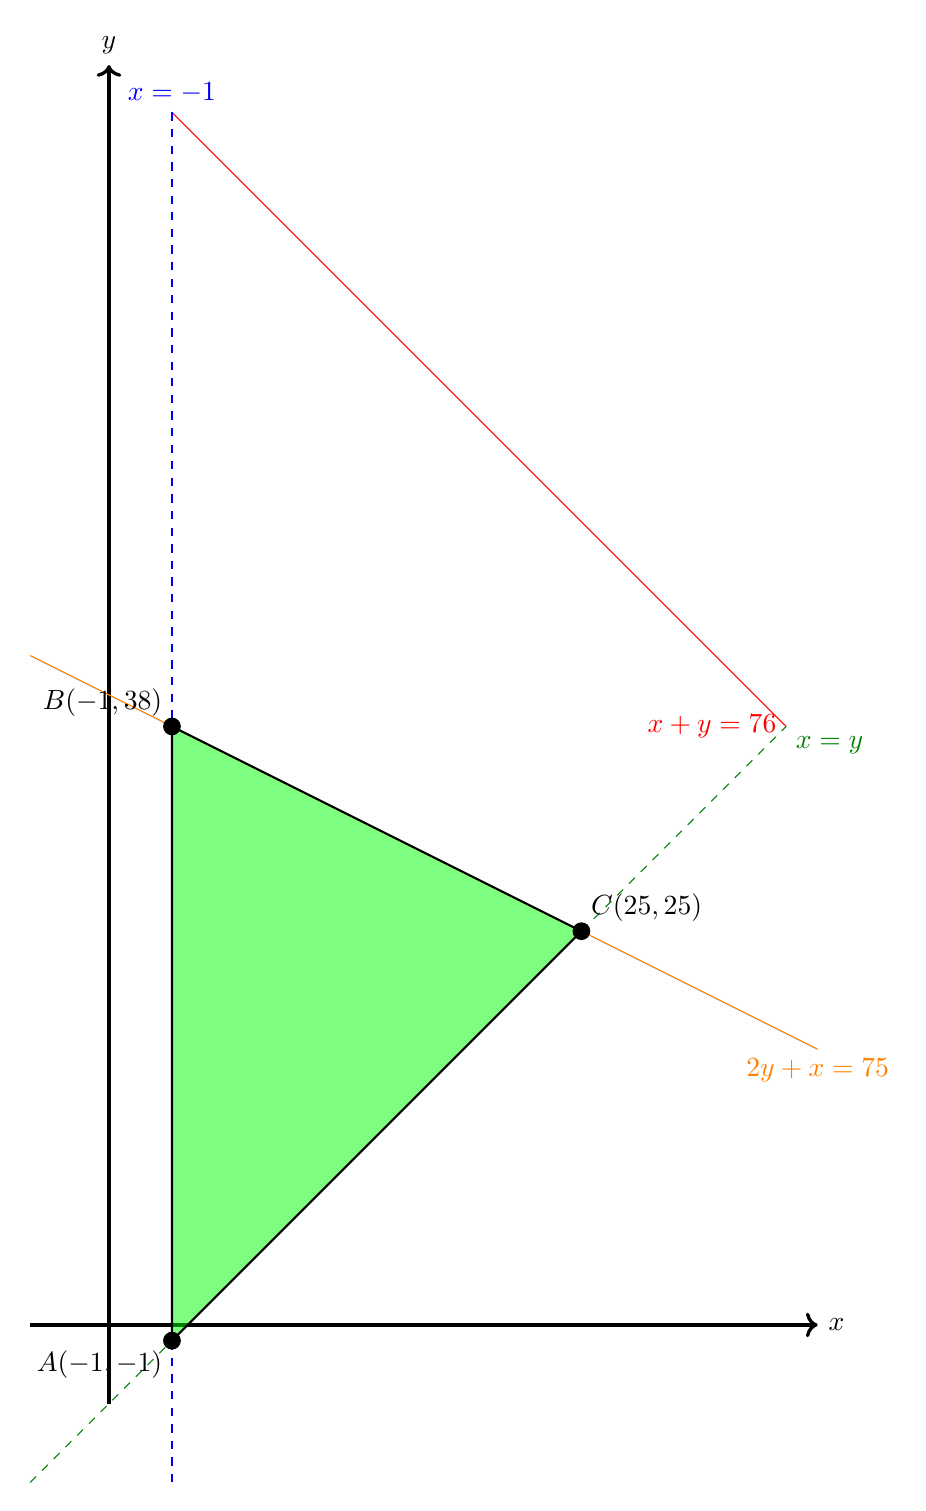
\begin{tikzpicture}[x=0.2cm,y=0.2cm]

    \draw[very thick,->] (-10,0) -- (40,0) node[right] {$x$};
    \draw[very thick,->] (-5,-5) -- (-5,80) node[above] {$y$};
    
    \draw[red] (-1,77) -- (38,38) node[left, sloped] {$x+y=76$};
  
  % Line 2: x=-1  (blue, dashed)
    \draw[dashed,blue] (-1,-10) -- (-1,77) node[above] {$x=-1$};
    
    % Line 3: x=y  (green!50!black, dashed)
    \draw[dashed,green!50!black] (-10,-10) -- (38,38) node[below right,sloped] {$x=y$};
    
    % Line 4: 2y+x=75  (orange, dashed)
    % Note: 2y+x=75  ⟺  y = (75-x)/2.
    \draw[orange] (-10,42.5) -- (40,17.5) node[below,sloped] {$2y+x=75$};
    
    % Fill the bounded (finite) region in green.
    % (This is the triangle with vertices A=(-1,-1), B=(-1,38), C=(25,25).)
    \fill[green,opacity=0.5] (-1,-1) -- (-1,38) -- (25,25) -- cycle;
    
    % Draw the triangle boundary a bit thicker.
    \draw[thick] (-1,-1) -- (-1,38) -- (25,25) -- cycle;
    
    % Mark and label the vertices.
    \filldraw[black] (-1,-1) circle (3pt) node[below left] {$A(-1,-1)$};
    \filldraw[black] (-1,38) circle (3pt) node[above left] {$B(-1,38)$};
    \filldraw[black] (25,25) circle (3pt) node[above right] {$C(25,25)$};

\end{tikzpicture}\\

The region with finite area is bounded by $A(-1, -1)$, $B(-1, 38)$, and $C(25, 25)$. \\Substituting $z=75-x-y$, we find that the area in the $xyz$ plane is bounded by $A(-1, -1, 77)$, $B(-1, 38, 38)$, and $C(25, 25, 25)$. By the Pythagorean theorem, $AB=39\sqrt{2}$, $BC=13\sqrt{6}$, and $AC=26\sqrt{6}$. This is a $30-60-90$ triangle with right angle at $B$, therefore, the area is $$\frac{39\sqrt{2}\cdot13\sqrt{6}}{2} = 507\sqrt{3} = \boxed{510}$$

I failed to recognize how straightforward this was and guessed on this one :(

\newpage

\section*{Problem 13}

\textbf{Alex divides a disk into four quadrants with two perpendicular diameters intersecting at the center of the disk. He draws $25$ more lines segments through the disk, drawing each segment by selecting two points at random on the perimeter of the disk in different quadrants and connecting these two points. Find the expected number of regions into which these $27$ line segments divide the disk.}

\newpage

\section*{Problem 14}

\textbf{Let $ABCDE$ be a convex pentagon with $AB=14,$ $BC=7,$ $CD=24,$ $DE=13,$ $EA=26,$ and $\angle B=\angle E=60^{\circ}.$ For each point $X$ in the plane, define $f(X)=AX+BX+CX+DX+EX.$ The least possible value of $f(X)$ can be expressed as $m+n\sqrt{p},$ where $m$ and $n$ are positive integers and $p$ is not divisible by the square of any prime. Find $m+n+p.$}

\newpage

\section*{Problem 15}

\textbf{Let $N$ denote the numbers of ordered triples of positive integers $(a, b, c)$ such that $a, b, c \le 3^6$ and $a^3 + b^3 + c^3$ is a multiple of $3^7$. Find the remainder when $N$ is divided by $1000$.}

We proceed with lifting the exponent. 
\end{document}
